\PassOptionsToPackage{unicode=true}{hyperref} % options for packages loaded elsewhere
\PassOptionsToPackage{hyphens}{url}
%
%\documentclass[120pt]{article}
\documentclass[a4paper, 12pt]{extarticle}

\usepackage{lmodern}
\usepackage{amssymb,amsmath}
\usepackage{ifxetex,ifluatex}
\usepackage{fixltx2e} % provides \textsubscript
\ifnum 0\ifxetex 1\fi\ifluatex 1\fi=0 % if pdftex
  \usepackage[T1]{fontenc}
  \usepackage[utf8]{inputenc}
  \usepackage{textcomp} % provides euro and other symbols
\else % if luatex or xelatex
  \usepackage{unicode-math}
  \defaultfontfeatures{Ligatures=TeX,Scale=MatchLowercase}
\fi
% use upquote if available, for straight quotes in verbatim environments
\IfFileExists{upquote.sty}{\usepackage{upquote}}{}
% use microtype if available
\IfFileExists{microtype.sty}{%
\usepackage[]{microtype}
\UseMicrotypeSet[protrusion]{basicmath} % disable protrusion for tt fonts
}{}
\IfFileExists{parskip.sty}{%
\usepackage{parskip}
}{% else
\setlength{\parindent}{0pt}
\setlength{\parskip}{6pt plus 2pt minus 1pt}
}
\usepackage{hyperref}
\hypersetup{
            pdfborder={0 0 0},
            breaklinks=true}
\urlstyle{same}  % don't use monospace font for urls
\usepackage{longtable,booktabs}
% Fix footnotes in tables (requires footnote package)
\IfFileExists{footnote.sty}{\usepackage{footnote}\makesavenoteenv{longtable}}{}
\setlength{\emergencystretch}{3em}  % prevent overfull lines
\providecommand{\tightlist}{%
  \setlength{\itemsep}{0pt}\setlength{\parskip}{0pt}}
\setcounter{secnumdepth}{0}
% Redefines (sub)paragraphs to behave more like sections
\ifx\paragraph\undefined\else
\let\oldparagraph\paragraph
\renewcommand{\paragraph}[1]{\oldparagraph{#1}\mbox{}}
\fi
\ifx\subparagraph\undefined\else
\let\oldsubparagraph\subparagraph
\renewcommand{\subparagraph}[1]{\oldsubparagraph{#1}\mbox{}}
\fi

% set default figure placement to htbp
\makeatletter
\def\fps@figure{htbp}
\makeatother

% Color links in blue
\usepackage{hyperref}
\hypersetup{
    colorlinks = true,
    citecolor = {black},
    linkcolor = {black},
    urlcolor = {blue}}

\usepackage{graphicx}
\graphicspath{ {/img/} }
%% Bold figure number
\usepackage[labelfont=bf]{caption}
%% Cite as superscript
\usepackage[super,square]{natbib}
%%%%%%%%%%%%%%%%%%%%%%%%%%%%%%%%%%%%%%%%%%%%%%%%
% Set Helvetica Font in Text and Math in LaTeX %
%%%%%%%%%%%%%%%%%%%%%%%%%%%%%%%%%%%%%%%%%%%%%%%%
\renewcommand{\familydefault}{\sfdefault}
\usepackage[scaled=1]{helvet}
\usepackage[helvet]{sfmath}
\everymath={\sf}
%% Set spacing to 1.5
\renewcommand{\baselinestretch}{1.4}
%% Set margins
\usepackage[legalpaper, margin=1.3in]{geometry}

\begin{document}

\renewcommand{\contentsname}{Table of Contents}
\newpage
  \tableofcontents
\newpage

\hypertarget{introduction}{%
\section{Introduction}\label{introduction}}

Safety is the most essential priority while driving with US drivers
considering safety the most influential point when purchasing a car
\cite{statista_global_2020}. One of the major factors reducing safety
for both drivers and pedestrians is drowsiness behind the wheel. It has
been demonstrated to severely impair driving performance. On average,
tired drivers perform worse than alcohol-intoxicated individuals with a
blood alcohol concentration of 0.05\% \cite{williamson_moderate_2000}.
Drowsiness is also the main cause of about 17\% of fatal traffic
accidents  \cite{tefft_prevalence_2010}.

In the US alone about \$671 Billion worth of goods per year are
transported by 15 million trucks
\cite{bureau_of_transportation_statistics_freight_2017}. The monetary
loss due to crashes has been growing steadily since 2013. In 2016,
crashes involving large trucks and busses leading to property damage,
injury and fatalities, amounted to a total loss of \$134 Billion
\cite{federal_motor_carrier_safety_administration_pocket_2018}.
Predicting dangerous levels of tiredness and preventing crashes and
accidents offers an opportunity to produce safer vehicles that in turn
will increase their value to potential car buyers.

This white paper analyses the current research available on patterns of
drowsiness that can lead to vehicle accidents, as well as current and
future solutions to the problem.

\hypertarget{drowsiness}{%
\section{1. Drowsiness}\label{drowsiness}}

Drowsiness is the tendency of an individual to fall asleep. There are
three main phases of sleep: awake, Non-Rapid Eye Movement (NREM) sleep
and Rapid Eye Movement (REM) sleep \cite{brodbeck_eeg_2012}. NREM can
then be subdivided three stages by using brain waves data from
electroencephalograms (EEG):

\begin{itemize}
\tightlist
\item
  Stage 1: Awake to Asleep transition (drowsy)
\item
  Stage 2: Light Sleep
\item
  Stage 3: Deep Sleep
\end{itemize}

Drowsiness-related accidents show recurring characteristics. They occur
primarily late at night (0:00 AM -- 7:00 AM) or in the early afternoon
(2:00 PM -- 4:00 PM). Usually, there are no signs of vehicle defects or
breaks usage and the weather conditions are generally good with clear
visibility \cite{sahayadhas_detecting_2012}. Multiple studies
\cite{philip_fatigue_2005} \cite{thiffault_monotony_2003} have
identified the monotony of the road environment as a possible trigger
for drowsiness. Moreover, signs of drowsiness based on the drivers'
performance can be observed within 20-25 minutes of driving
\cite{philip_fatigue_2005}.

Additionally, the European Road Safety Observatory identified the lack
of sleep, time spent on a task, monotony of the road and the internal
body clock, as main sources of drowsiness that can lead to fatal
accidents\cite{european_commission_fatigue_2018}.


\hypertarget{measuring-drowsiness}{%
\section{2. Measuring Drowsiness}\label{measuring-drowsiness}}

Drowsiness detection systems typically attempt at detecting the early
stages of NREM. They generally consist of a device that is embedded in
the vehicle and monitors the driver. The device captures data in the
form of pictures from a camera or sensors such as steering wheel
sensors. The data is then processed and analyzed by an algorithm to
measure the drowsiness level. This process can be repeated multiple
times for a certain length of time \texttt{t} Figure \ref{fig:detection}.



\begin{figure}[ht]
    \centering
    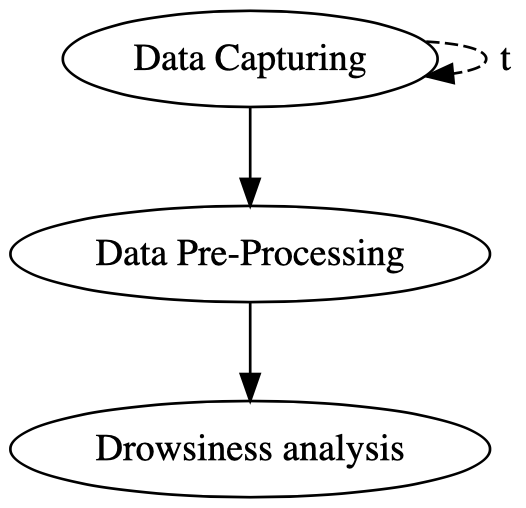
\includegraphics[width=0.4\textwidth]{img/detection.png}
    \caption{A diagrammatic representation of the
drowsiness analysis process. When data is recorded, it is then
pre-processed and used for drowsiness analysis. The process is usually
repeated over time (dashed line labeled \texttt{t}).}
    \label{fig:detection}
\end{figure}

This process is adapted in different ways depending on the type of data
being collected, which is either: subjective, vehicle-based, behavioral
or physiological.

\hypertarget{subjective-measures}{%
\subsection{2.1 Subjective Measures}\label{subjective-measures}}

Subjective measures involve the driver's assessment of their alertness
level. The Karolinska Sleepiness Scale (KSS) is a nine-point scale and
it is the most widely used scales to describe drowsiness
\cite{shahid_karolinska_2012}. Each rating of the KSS has an associated
description as shown in Table \ref{table:karolinska}.
\newpage
\begin{longtable}[ht]{@{}ll@{}}
\toprule
\textbf{Rating} & \textbf{Description}\tabularnewline
\midrule
\endhead
1 & Extremely alert\tabularnewline
2 & Very alert\tabularnewline
3 & Fairly alert\tabularnewline
4 & Alert\tabularnewline
5 & Neither alert nor sleepy\tabularnewline
6 & Some signs of sleepiness\tabularnewline
7 & Sleepy but no effort to keep alert\tabularnewline
8 & Sleepy some effort to keep alert\tabularnewline
9 & Very Sleepy, great effort to keep alert, fighting
sleep\tabularnewline
\bottomrule
\caption{The Karolinska Sleepiness Scale (KSS) with
descriptions for each rating.}
\label{table:karolinska}
\end{longtable}

The KSS has been used to monitor the driver's drowsiness level in
driving simulations and compared to other sources of data such as EEG
data \cite{hu_driver_2009} or Lane Position data
\cite{golz_evaluation_2010}.

The results, however, were mixed and they largely depend on the driver's
consistency in the self-assessment. This method may not be consistent
between different drivers and may also fail to capture sudden changes in
drowsiness levels due to microsleep events. An additional limitation it
is difficult to inquire about the driver while driving on a real road,
and in addition to being a source of distraction, it may indirectly
alert the driver, affecting their drowsiness level
\cite{sahayadhas_detecting_2012}.

\hypertarget{vehicle-based-measures}{%
\subsection{2.2 Vehicle-Based Measures}\label{vehicle-based-measures}}

Vehicle-based measures aim at determining the drowsiness level via the
interaction between the driver and the vehicle. These usually involve
sensors such as steering wheel sensors or lane position sensors.

\hypertarget{steering-wheel-sensors}{%
\subsubsection{Steering Wheel Sensors}\label{steering-wheel-sensors}}

These sensors measure the change in the angle of the steering wheel.
There are two main phases of drowsiness that can be detected with
steering wheel sensors:

\begin{itemize}
\tightlist
\item
  \textbf{Phase 1}: Early-stage drowsiness where the driver is unable to
  smoothly control the vehicle, with large maneuvers to correct the
  vehicle position. This usually results in zigzag driving and has been
  reported by multiple research. Studies\cite{sayed_unobtrusive_2001}
  \cite{eskandarian_evaluation_2007}
\item
  \textbf{Phase 2}: The dozing off phase. The driver stops reacting to
  feedback from the road, therefore the steering sensors have a flat and
  constant value which is usually combined with an increased lateral
  position \cite{eskandarian_evaluation_2007}.
\end{itemize}

Typically, these two phases alternate each other in drowsy individual,
right before a crash (Figure \ref{fig:steering})

\begin{figure}[ht]
    \centering
    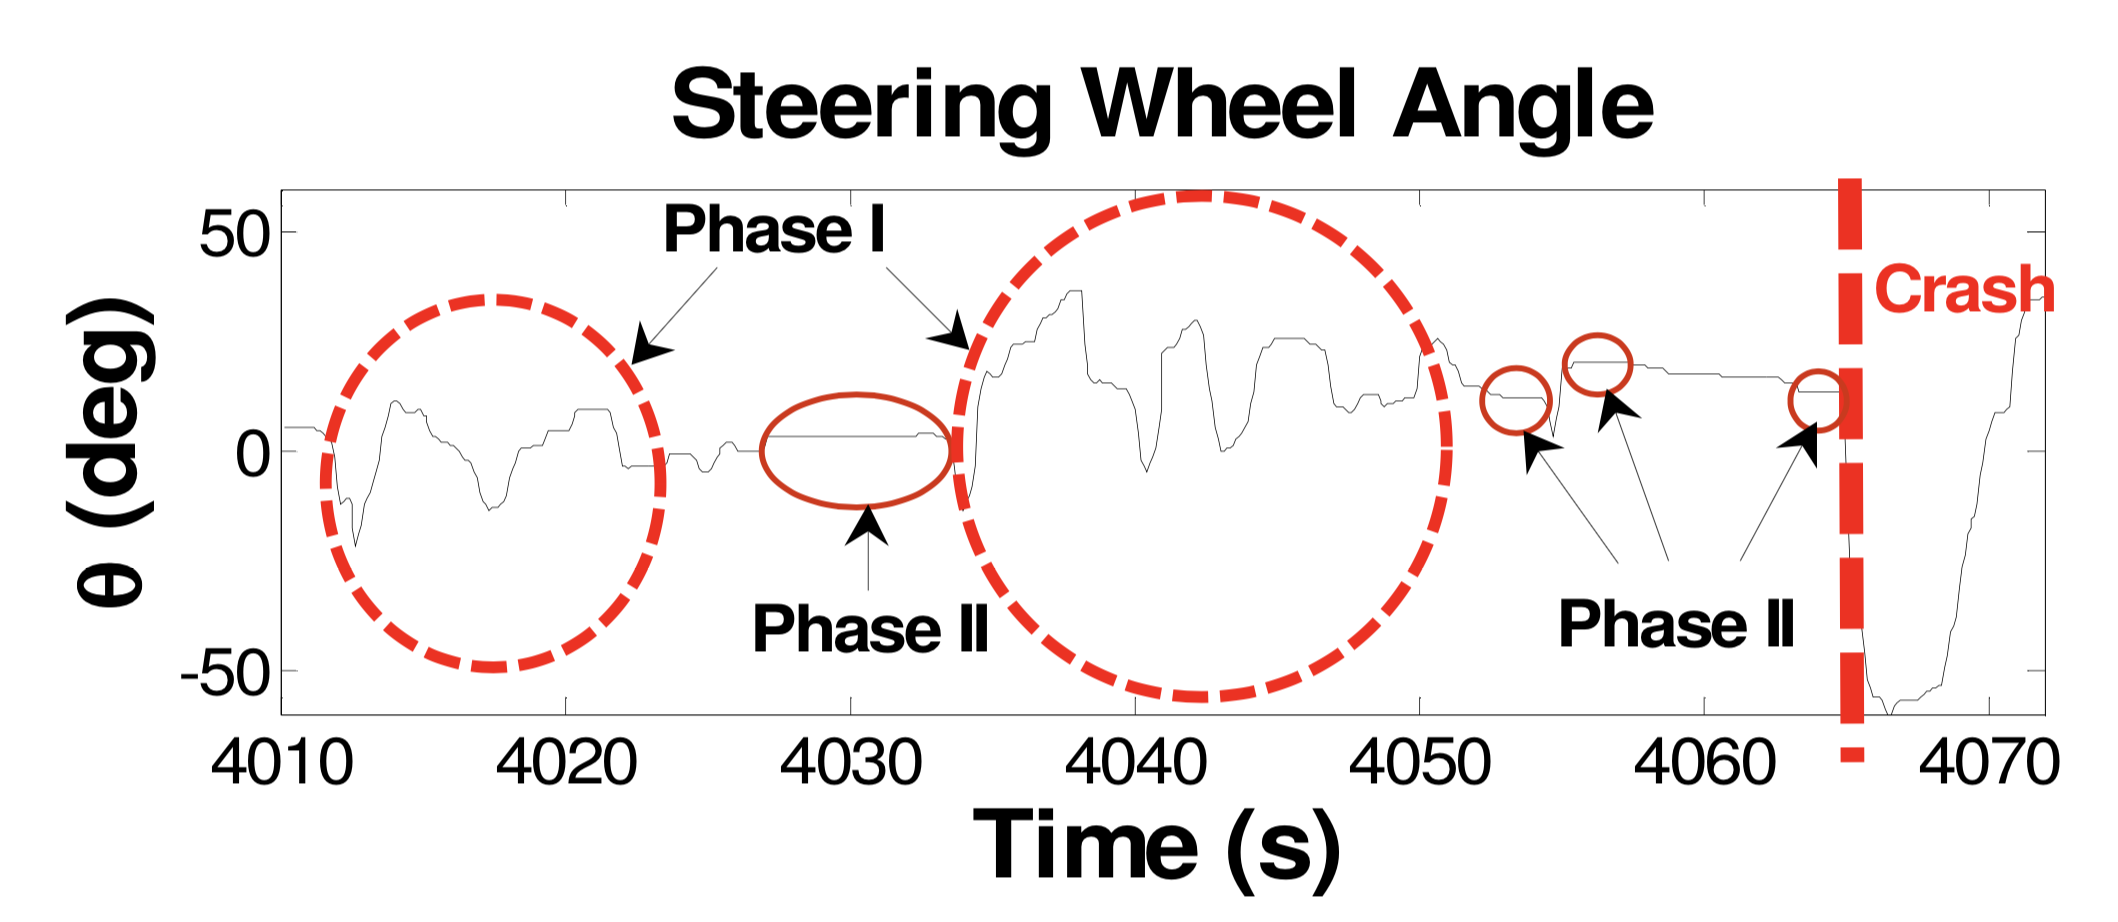
\includegraphics[width=0.9\textwidth]{img/steering.png}
    \caption{Steering wheel angle patterns in a 5 km drive
simulation. There are two main phases: Phase 1 characterized by large
changes in steering angles and Phase 2 with rather constant values.
\cite{eskandarian_evaluation_2007}}
    \label{fig:steering}
\end{figure}


Other measures that can be calculated from steering sensors are the
Standard Deviation of Angular Velocity (SDAV) of the steering wheel and
the proportion of STeering wheel movements EXceeding Three degrees
(STEX3). These are highly correlated to Psychomotor Vigilance Tests and
the KSS scale. \cite{forsman_efficient_2013}

These sensors work optimally with steering angles between 0.5° - 5.0°
and they are also relatively easy to install on vehicles. Steering wheel
metrics, however, are too dependent on roads with specific geometries
and may be affected by the vehicle kinetics in particular environments.
Additionally, monotonous roads such as straight roads, provide little to
no variation to be detected which may result in drowsiness not being
detected. Steering wheel sensors may also fail to detect changes in
relatively straight roads or highly trafficked roads, which are among
the roads with the highest number of accidents.
\cite{eskandarian_evaluation_2007}

\hypertarget{lane-position-sensors}{%
\subsubsection{Lane Position Sensors}\label{lane-position-sensors}}

Lane position sensors involve a combination of an external camera and
lane-tracking algorithms to calculate the position of the vehicle with
respect to the lanes.

Patterns that can be calculated from this type of data are Standard
Deviation of Lane Position (SDLP) \cite{ingre_subjective_2006}, Lateral
Lane Position \cite{cheng_driver_2012} and the Frequency of Abnormal
Lane Deviation \cite{hu_experimental_2017}. In their research, Ingre et
al. \cite{ingre_subjective_2006} found a significant correlation between
the KSS scale and both the SDLP (Figure\ref{fig:lane_position}) and the blink duration
which is also discussed in the next section.

\begin{figure}[ht]
    \centering
    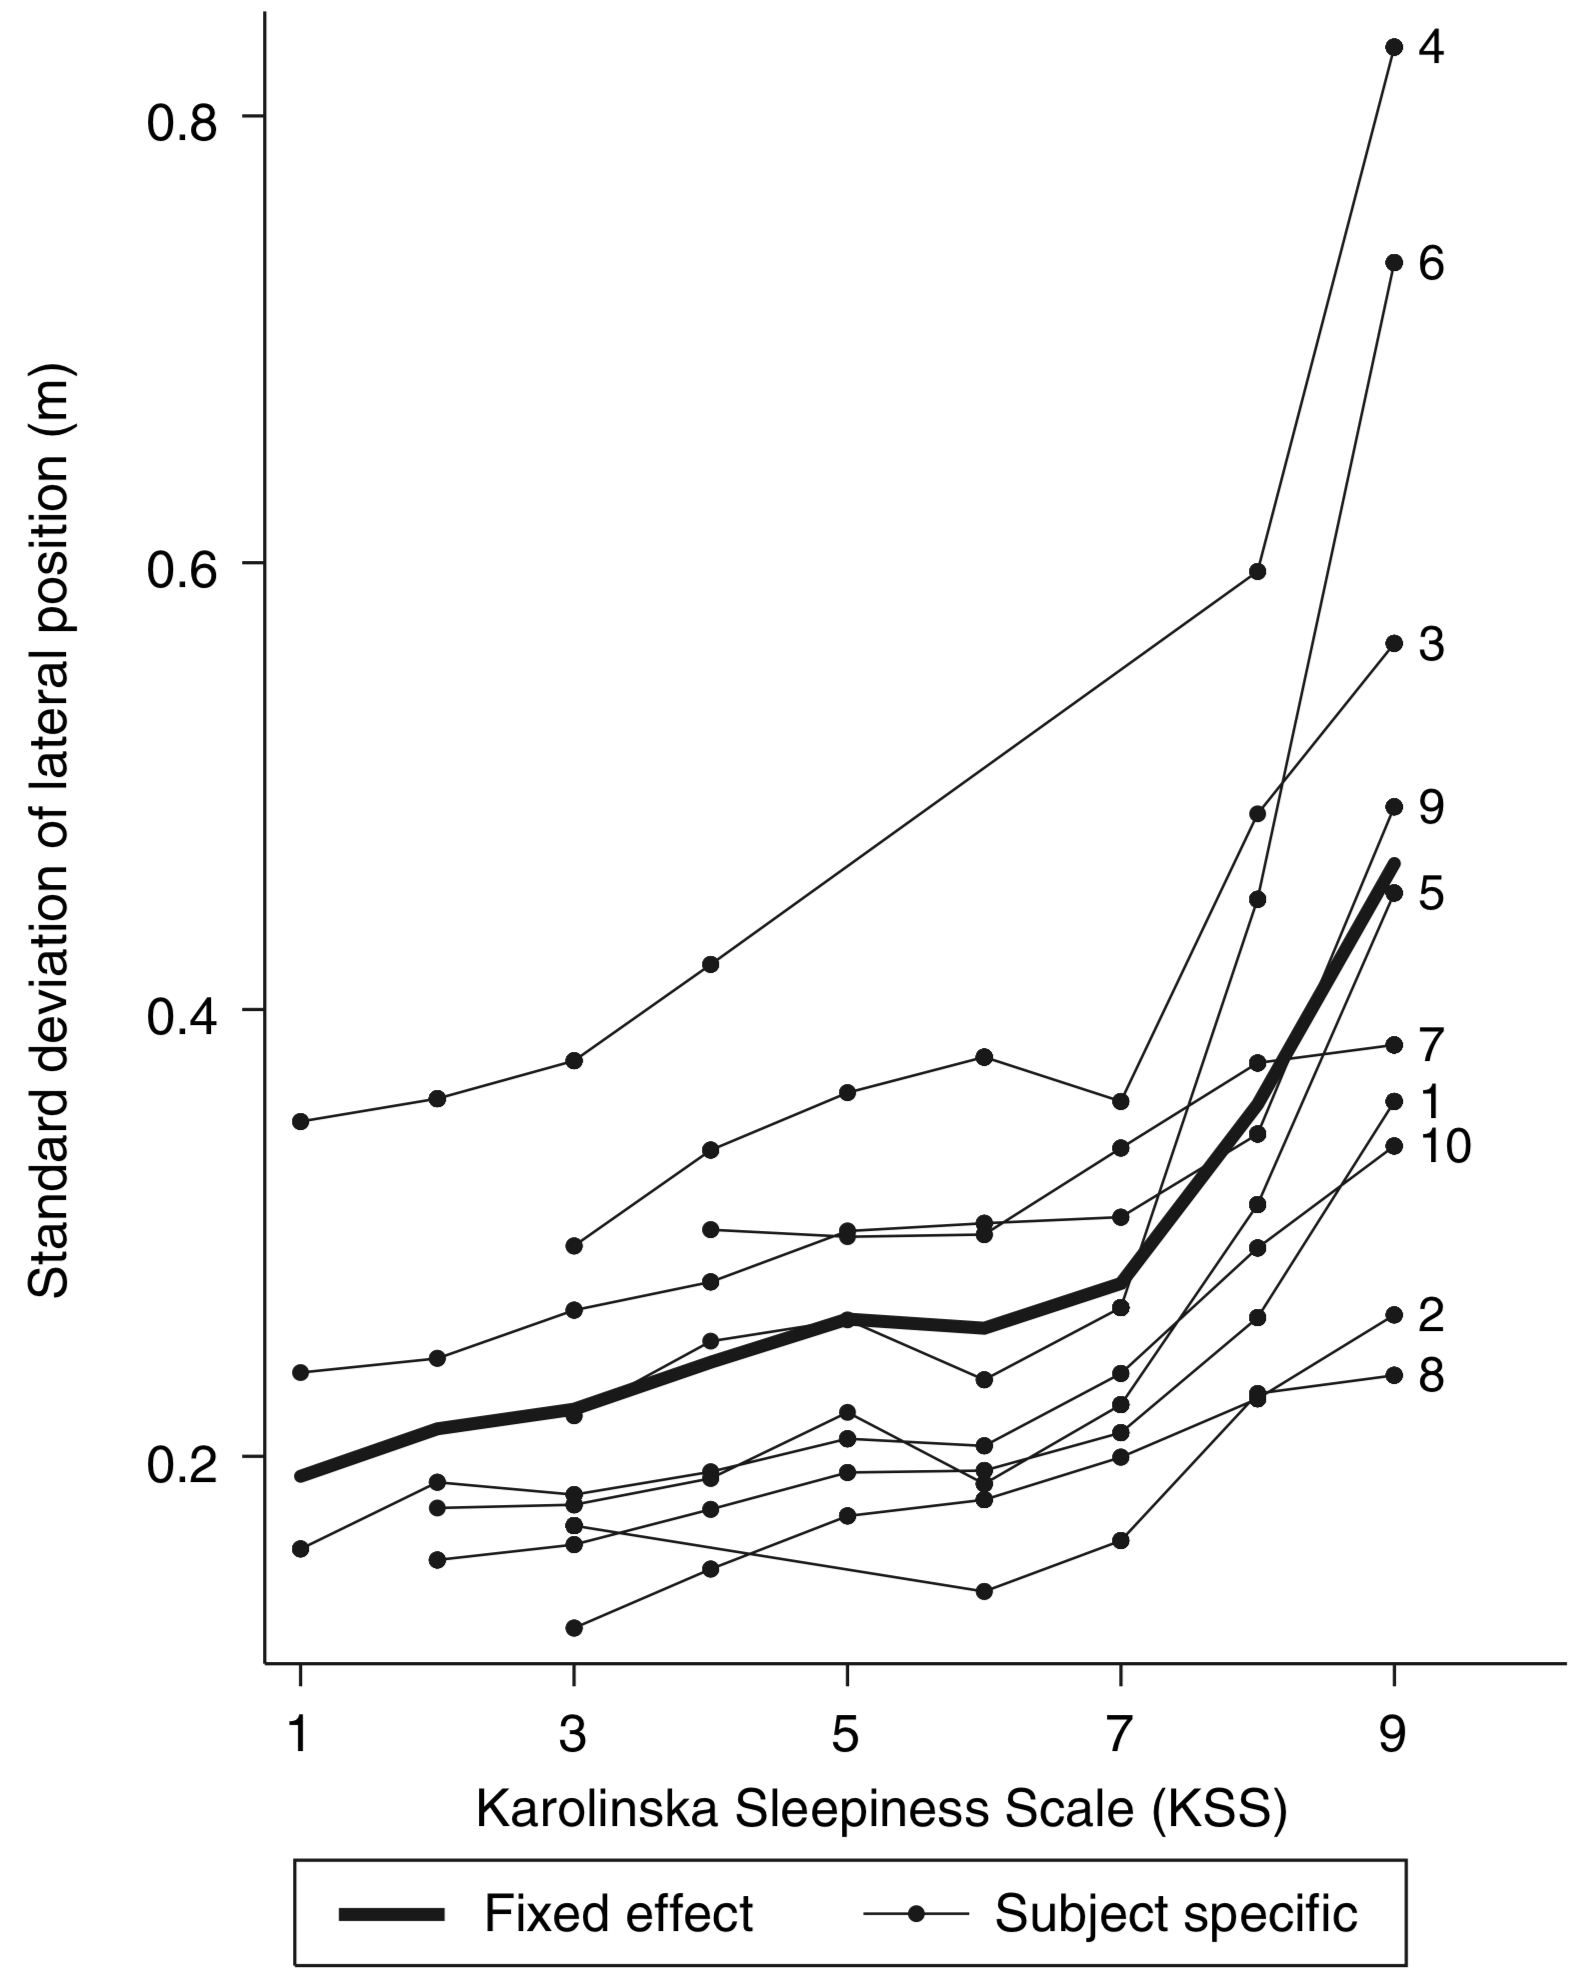
\includegraphics[width=0.8\textwidth]{img/lane_position.png}
    \caption{A positive correlation between the Standard
Deviation of Lane Position (SDLP) and the Karolinska Sleepiness Scale
(KSS) (n = 20). The estimated fixed effect (thick) shows a peak in
drowsiness (KSS 8-9) between SDLP of 0.36 and 0.40 \cite{ingre_subjective_2006}. }
    \label{fig:lane_position}
\end{figure}

Limitations of this method include the dependency on road marks for lane detection, lighting and weather
conditions \cite{sahayadhas_detecting_2012}.

\hypertarget{behavioural-measures}{%
\subsection{2.3 Behavioural Measures}\label{behavioural-measures}}

Behavioral measures attempt at identifying behaviors associated with
drowsiness. They usually rely on a camera that records the driver's
face. A set of features is extracted from the pictures which can be
correlated to drowsiness (e.g.~eyes closed for a prolonged period of
time). The majority of the features are obtained from the mouth, eyes,
or head as a whole.

\hypertarget{mouth-features}{%
\subsubsection{Mouth Features}\label{mouth-features}}

Yawns are the most common mouth features correlated with drowsiness.
This is usually measured as the degree of mouth openness which will vary
if the driver is normal, drowsy or just talking
\cite{qiong_wang_driver_2006}.

\hypertarget{eyes-features}{%
\subsubsection{Eyes Features}\label{eyes-features}}

Eyes, and more specifically blinking, have been studied extensively for
drowsiness detection. The most commonly used approach is PERCLOS, the
PERcentage of eyes CLOSure over a time period and is very effective in
drowsiness detection \cite{sahayadhas_detecting_2012}. A more recent
study by Trutschel et al. \cite{trutschel_perclos:_2011} however,
challenged the effectiveness of PERCLOS and commercially available
PERCLOS-based systems. In a trial with three commercial systems, PERCLOS
had a higher error rate in drowsiness detection of about 10\% compared
to EEG data. This has been associated with episodes of microsleep events
where drivers are asleep with their eyes open which PERCLOS fails to
address.

Alternative eye features correlated with drowsiness include the Average
Eye Closure Speed (AECS), Blink Frequency and Duration and pupil
diameter. Additionally, eye gaze can also be extracted to verify whether
the driver is looking at the road ahead \cite{qiong_wang_driver_2006}.

\hypertarget{head-features}{%
\subsubsection{Head Features}\label{head-features}}

Drowsy drivers seem to sway their heads, increase nodding, scratch their
faces more frequently and more prone to rotate their heads to the left
to relieve tension on the neck. The head position can also be used to
calculate the slouching and posture adjustment frequency. The features
involving rotations are quantifiable with available face detection
methods. Other behaviors like scratching may be harder to quantify and
may not be consistent across different individuals.
\cite{eskandarian_evaluation_2007}

Once these features are extracted, a threshold is set to classify the
driver as drowsy or not. Given that most of these features rely on a
temporal dimension, they tend to perform better when used for a longer
period \cite{wilkinson_accuracy_2013}.

The main limitation of behavioral approaches is the camera as it is
significantly affected by light conditions. This has partially been
minimized by the addition of an infrared camera
\cite{sahayadhas_detecting_2012}. However, the systems may still be
sensitive to sudden changes in illumination or dust accumulating on the
camera sensor which may affect the feature detection steps.

\hypertarget{biological-measures}{%
\subsection{2.4 Biological Measures:}\label{biological-measures}}

Biological measures focus on detecting significant changes in
physiological signals as measured by electrocardiogram (ECG),
electroencephalogram (EEG), electro-oculography (EOG), surface
electromyogram (sEMG) \cite{dong_driver_2011}.

EEG has been studied extensively, as it detects brain waves related to
sleep \cite{qiong_wang_driver_2006}. Drowsiness is usually correlated
with an increase of a continuous signal of \(\alpha\) and \(\theta\)
waves compared to \(\beta\) waves, detectable over a time period of choice with the formula:

\[ \dfrac{\Delta \alpha + \Delta \theta}{\Delta \beta} \]

Although very accurate, EEG measurements are very invasive, consisting
of electrodes in contact with the skin \cite{dong_driver_2011}.
Nonetheless, it has been very useful to evaluate other patterns of
drowsiness such as Standard Deviation of Steering Wheel Angle and
Lateral Lane Position \cite{boyle_driver_2008}.

\hypertarget{hybrid-measures}{%
\subsection{2.5. Hybrid measures}\label{hybrid-measures}}

Theoretically, combining information about the driver's physical state
and driving performance should improve the confidence of the detected
fatigue \cite{dong_driver_2011}. Hybrid measures consider multiple
patterns of drowsiness, such as the ones previously outlined, to refine
the confidence of the prediction.

As an example, Eskandarian and colleagues analyzed driving data from 20
subjects over two days. The study identified correlations between
PERCLOS, Steering Wheel Angle, Lateral Displacement of the vehicle and
vehicle crash accidents. A neural network model trained on all of these
patterns achieved a larger accuracy with lower false-positive signals
compared to just considering one pattern \cite{eskandarian_evaluation_2007}.

Machine learning models are therefore suitable candidates for drowsiness
detection solutions for three main reasons: personalization, accuracy,
and versatility.

\begin{itemize}
\item
  \textbf{Personalization:} Unlike many patterns of tiredness described
  earlier such as PERCLOS, machine learning does not rely on specific
  values to determine the drowsiness. Instead, machine learning can
  \emph{learn} drowsiness-specific patterns on a driver-to-driver basis,
  taking into account variations in the individuals.
\item
  \textbf{Accuracy:} Additionally, machine learning models can improve
  their accuracy as more data from the driver is obtained compared to
  other algorithms. Their great versatility also allows them
\item
  \textbf{Versatility:} Due to their modular architecture, machine
  learning models allow for multiple sources of data to be used, as in
  the case of Eskandarian and colleagues Additionally, this allows
  adaptation to data from new sensors that may be developed in the
  future.
\end{itemize}

In terms of drawbacks, machine learning models generally take longer
development time, as they need to be trained with appropriate datasets
and require hyperparameters tuning. Additionally, even high-accuracy
machine learning models tend to have black-box properties, meaning it
may be hard to understand exactly how they reached their conclusions.
Finally, high-accuracy models are usually resource-intensive which means
they require high computational power to be trained.

\hypertarget{proposed-solution}{%
\section{3. Proposed Solution}\label{proposed-solution}}

Osmitau Technologies is tackling these problems to create a hybrid
solution called Teyered, powered by machine learning:

\begin{itemize}
\item
  \textbf{Development Time}: Osmitau's team has had extensive experience
  in the fields of machine learning and data analysis, working at
  companies such as IBM, JPMorgan, and Amazon. They take care of the
  development for you.
\item
  \textbf{Explainability}: Teyered does not uniquely rely on
  off-the-shelf black-box models. It exploits advanced statistical
  methods to extract relevant patterns from drivers' data and couples
  them with an advanced prediction model to determine the drowsiness
  state of the driver.
\item
  \textbf{Computational Power:} Osmitau takes care of the computational
  resources required for training the system by using the best
  high-performance cloud computing platforms provided by Google (GCP)
  and Amazon (AWS). This approach guarantees fast training times and the
  immediate availability of resources.
\end{itemize}

\hypertarget{conclusion}{%
\section{4. Conclusion}\label{conclusion}}

Truck and bus accidents result in a loss of \$134 Billion which includes
property damage, injury and fatalities
\cite{federal_motor_carrier_safety_administration_pocket_2018}. More
than 40\% of accidents involving commercial vehicles occur due to
drowsiness \cite{flatley_sleep-related_2004} and it manifests itself in
several detectable patterns that are used in current
drowsiness-detection systems. The patterns most correlated with
drowsiness involve vehicle sensors such as steering wheel angle and
driver's behavior such as blinking rate. Other physiological indicators
such as EEG waves, although accurate, are invasive to the driver but can
be used as a baseline to validate other potential signs of tiredness.

Nevertheless, the most accurate methods for drowsiness detection involve
the use of multiple patterns as an input to the predictive system into a
hybrid solution. This can be done using a statistical method with a
fixed drowsiness threshold, an adaptive black-box machine learning or a
combination of the two.

\hypertarget{find-out-more}{%
\subsection{Find out more}\label{find-out-more}}

You can find out more about our company and our services at
\url{www.osmitau.com}. We offer consulting services for AI and Machine
Learning and can help you tackle complex problems that require optimal
solutions.

Osmitau is aiming to release Teyered in early 2020. You can join our newsletter by clicking \href{http://eepurl.com/gO-J9n}{HERE} (we don't spam, unlike the big guys).

Or you can email us at \href{mailto:hello@osmitau.com}{\nolinkurl{hello@osmitau.com}}.

\addcontentsline{toc}{section}{References}
\bibliographystyle{plain}
\bibliography{refs.bib}

\newpage

Special thanks to Eric Weber for the photograph on the cover of this
white paper.

\vspace*{\fill}
\textbf{Notice:}  

ALL INFORMATION PROVIDED IN THIS WHITE PAPER IS PROVIDED ``AS
IS''. OSMITAU TECHNOLOGIES MAKES NO WARRANTIES, EXPRESSED, IMPLIED,
STATUTORY OR OTHERWISE WITH RESPECT TO THE MATERIALS, AND EXPRESSLY
DISCLAIMS ALL IMPLIED WARRANTIES OF NON-INFRINGEMENT, MERCHANTABILITY,
AND FITNESS FOR A PARTICULAR PURPOSE.


Information furnished is believed to be accurate and reliable. However,
Osmitau Technologies assumes no responsibility for the consequences of
use of such information or for any infringement of patents or other
rights of third parties that may result from its use. No license is
granted by implication or otherwise under any patent or patent rights of
Osmitau Technologies. Specifications mentioned in this publication are
subject to change without notice. This publication supersedes and
replaces all information previously supplied.

This document was last updated on \today.

\newpage
\end{document}